\documentclass[12pt, xcolor=table]{beamer}
\usepackage{graphicx}
\usepackage[ngerman]{babel}
\usepackage[utf8]{inputenc}
\usepackage{amsmath}
\usepackage{amssymb}
\usepackage{listings}
\usepackage{hyperref}
\usepackage{fancyvrb}
\usepackage{color}
\usepackage{alltt}

\usepackage[percent]{overpic}
\usepackage[footnotesize, bf]{caption}
%Copyright 2008 by Adrian Böhmichen
%
% This file is free software: you can redistribute it and/or modify
% it under the terms of the GNU General Public License as published by
% the Free Software Foundation, either version 3 of the License, or
% (at your option) any later version.
%
% This file is distributed in the hope that it will be useful,
% but WITHOUT ANY WARRANTY; without even the implied warranty of
% MERCHANTABILITY or FITNESS FOR A PARTICULAR PURPOSE.  See the
% GNU General Public License for more details.
%
% You should have received a copy of the GNU General Public License
% along with this file.  If not, see <http://www.gnu.org/licenses/>.

%%%%%%%%%%%%%%%%%%%%%%%%%%%%%%%%%%%%%%%%%%%%%%%%%%%%%%%%%%%%%%%%%
%     Ubuntuusers Vorlage für ein LaTeX-Beamer Theme            %
%                                                               %
% Für das Korrekte funktionieren benötigt man einen header.png  %
% und ein logo.png Datei!                                       %
% Zusätzlich muss man folgende Pakete benutzten:                %
%   \usepackage{graphicx}                                       %
%   \usepackage[percent]{overpic}                               %
%                                                               %
% Danach muss nur noch am Anfang die Datei                      %
% mit \input{} eingebunden werden.                              %
%                                                               %
%%%%%%%%%%%%%%%%%%%%%%%%%%%%%%%%%%%%%%%%%%%%%%%%%%%%%%%%%%%%%%%%%

%weitere Farbe spezifizieren:
%Farben von dem Humantheme
%\definecolor{Orange}{RGB}{240,165,19}
\definecolor{Orange}{RGB}{5,215,242}
%\definecolor{Human-Base}{RGB}{129,102,71}
\definecolor{Human-Base}{RGB}{5,25,242}
%Farben aus dem Inyokatheme
%\definecolor{uuheader1}{RGB}{164,143,101}
\definecolor{uuheader1}{RGB}{5,25,242}
%\definecolor{uuheader2}{RGB}{129,106,59}
\definecolor{uuheader2}{RGB}{5,25,242}


%Theme festlegen für alle Templates die nicht selbstständig definiert werden:
\usepackage{beamerthemedefault}


%Definieren des Innertheme, zuständig für die Symbole bei Listen
\setbeamertemplate{sections/subsections in toc}[square]
\setbeamertemplate{items}[circle]

\setbeamercolor{item}{fg=Human-Base}

%entfernen der Navigationsleiste
\beamertemplatenavigationsymbolsempty

%Logo definieren, man kann die Lage nicht verändern
%\logo{\includegraphics[scale=0.1]{logo.png}}


%Kopf- und Fußzeile definieren
%\setbeamertemplate{headline}
%{%
%\begin{overpic}[width=\paperwidth
% nächste Zeile dient zum anzeigen eines Rasters, für das paltzieren des ToC hilfreich
%,grid,tics=10
%]
%{header.png}%
%  \put(0,11){\insertsectionnavigationhorizontal{\paperwidth}{~}{~}}%
%  \end{overpic}
%}

\setbeamertemplate{footline}[text line]
{%
\begin{minipage}[b]{116mm}
\insertauthor \hfill%
%neue Navigationsleiste
 \insertframenumber ~/ \inserttotalframenumber\\[1ex]
\end{minipage}
}

% Farben festlegen ausserhalb des innertheme

%Allgemeine Angaben und Verbesserung vom default Theme
\setbeamercolor{structure}{fg=uuheader1}
\setbeamercolor{section in toc}{fg=Human-Base}
\setbeamercolor{subsection in toc}{parent=section in toc}
\setbeamercolor{framesubtitle}{fg=uuheader2}


%Farbe und Form der Blöcke definieren
\setbeamertemplate{blocks}[rounded]
%\setbeamercolor{block title}{fg=uuheader1,bg=Orange}
%\setbeamercolor{block title alerted}{use=alerted text,fg=black,bg=alerted text.fg!75!bg}
%\setbeamercolor{block title example}{use=example text,fg=black,bg=example text.fg!75!bg}

%\setbeamercolor{block body}{parent=normal text,use=block title,bg=block title.bg!25!bg}
%\setbeamercolor{block body alerted}{parent=normal text,use=block title alerted,bg=block title alerted.bg!25!bg}
%\setbeamercolor{block body example}{parent=normal text,use=block title example,bg=block title example.bg!25!bg}

%Für den Titleframe
\setbeamertemplate{title page}[default][rounded=true]
\setbeamercolor{title}{fg=uuheader2,bg=Orange}


\makeatletter
\def\PY@reset{\let\PY@it=\relax \let\PY@bf=\relax%
    \let\PY@ul=\relax \let\PY@tc=\relax%
    \let\PY@bc=\relax \let\PY@ff=\relax}
\def\PY@tok#1{\csname PY@tok@#1\endcsname}
\def\PY@toks#1+{\ifx\relax#1\empty\else%
    \PY@tok{#1}\expandafter\PY@toks\fi}
\def\PY@do#1{\PY@bc{\PY@tc{\PY@ul{%
    \PY@it{\PY@bf{\PY@ff{#1}}}}}}}
\def\PY#1#2{\PY@reset\PY@toks#1+\relax+\PY@do{#2}}

\def\PY@tok@gd{\def\PY@tc##1{\textcolor[rgb]{0.63,0.00,0.00}{##1}}}
\def\PY@tok@gu{\let\PY@bf=\textbf\def\PY@tc##1{\textcolor[rgb]{0.50,0.00,0.50}{##1}}}
\def\PY@tok@gt{\def\PY@tc##1{\textcolor[rgb]{0.00,0.25,0.82}{##1}}}
\def\PY@tok@gs{\let\PY@bf=\textbf}
\def\PY@tok@gr{\def\PY@tc##1{\textcolor[rgb]{1.00,0.00,0.00}{##1}}}
\def\PY@tok@cm{\let\PY@it=\textit\def\PY@tc##1{\textcolor[rgb]{0.25,0.50,0.50}{##1}}}
\def\PY@tok@vg{\def\PY@tc##1{\textcolor[rgb]{0.10,0.09,0.49}{##1}}}
\def\PY@tok@m{\def\PY@tc##1{\textcolor[rgb]{0.40,0.40,0.40}{##1}}}
\def\PY@tok@mh{\def\PY@tc##1{\textcolor[rgb]{0.40,0.40,0.40}{##1}}}
\def\PY@tok@go{\def\PY@tc##1{\textcolor[rgb]{0.50,0.50,0.50}{##1}}}
\def\PY@tok@ge{\let\PY@it=\textit}
\def\PY@tok@vc{\def\PY@tc##1{\textcolor[rgb]{0.10,0.09,0.49}{##1}}}
\def\PY@tok@il{\def\PY@tc##1{\textcolor[rgb]{0.40,0.40,0.40}{##1}}}
\def\PY@tok@cs{\let\PY@it=\textit\def\PY@tc##1{\textcolor[rgb]{0.25,0.50,0.50}{##1}}}
\def\PY@tok@cp{\def\PY@tc##1{\textcolor[rgb]{0.74,0.48,0.00}{##1}}}
\def\PY@tok@gi{\def\PY@tc##1{\textcolor[rgb]{0.00,0.63,0.00}{##1}}}
\def\PY@tok@gh{\let\PY@bf=\textbf\def\PY@tc##1{\textcolor[rgb]{0.00,0.00,0.50}{##1}}}
\def\PY@tok@ni{\let\PY@bf=\textbf\def\PY@tc##1{\textcolor[rgb]{0.60,0.60,0.60}{##1}}}
\def\PY@tok@nl{\def\PY@tc##1{\textcolor[rgb]{0.63,0.63,0.00}{##1}}}
\def\PY@tok@nn{\let\PY@bf=\textbf\def\PY@tc##1{\textcolor[rgb]{0.00,0.00,1.00}{##1}}}
\def\PY@tok@no{\def\PY@tc##1{\textcolor[rgb]{0.53,0.00,0.00}{##1}}}
\def\PY@tok@na{\def\PY@tc##1{\textcolor[rgb]{0.49,0.56,0.16}{##1}}}
\def\PY@tok@nb{\def\PY@tc##1{\textcolor[rgb]{0.00,0.50,0.00}{##1}}}
\def\PY@tok@nc{\let\PY@bf=\textbf\def\PY@tc##1{\textcolor[rgb]{0.00,0.00,1.00}{##1}}}
\def\PY@tok@nd{\def\PY@tc##1{\textcolor[rgb]{0.67,0.13,1.00}{##1}}}
\def\PY@tok@ne{\let\PY@bf=\textbf\def\PY@tc##1{\textcolor[rgb]{0.82,0.25,0.23}{##1}}}
\def\PY@tok@nf{\def\PY@tc##1{\textcolor[rgb]{0.00,0.00,1.00}{##1}}}
\def\PY@tok@si{\let\PY@bf=\textbf\def\PY@tc##1{\textcolor[rgb]{0.73,0.40,0.53}{##1}}}
\def\PY@tok@s2{\def\PY@tc##1{\textcolor[rgb]{0.73,0.13,0.13}{##1}}}
\def\PY@tok@vi{\def\PY@tc##1{\textcolor[rgb]{0.10,0.09,0.49}{##1}}}
\def\PY@tok@nt{\let\PY@bf=\textbf\def\PY@tc##1{\textcolor[rgb]{0.00,0.50,0.00}{##1}}}
\def\PY@tok@nv{\def\PY@tc##1{\textcolor[rgb]{0.10,0.09,0.49}{##1}}}
\def\PY@tok@s1{\def\PY@tc##1{\textcolor[rgb]{0.73,0.13,0.13}{##1}}}
\def\PY@tok@sh{\def\PY@tc##1{\textcolor[rgb]{0.73,0.13,0.13}{##1}}}
\def\PY@tok@sc{\def\PY@tc##1{\textcolor[rgb]{0.73,0.13,0.13}{##1}}}
\def\PY@tok@sx{\def\PY@tc##1{\textcolor[rgb]{0.00,0.50,0.00}{##1}}}
\def\PY@tok@bp{\def\PY@tc##1{\textcolor[rgb]{0.00,0.50,0.00}{##1}}}
\def\PY@tok@c1{\let\PY@it=\textit\def\PY@tc##1{\textcolor[rgb]{0.25,0.50,0.50}{##1}}}
\def\PY@tok@kc{\let\PY@bf=\textbf\def\PY@tc##1{\textcolor[rgb]{0.00,0.50,0.00}{##1}}}
\def\PY@tok@c{\let\PY@it=\textit\def\PY@tc##1{\textcolor[rgb]{0.25,0.50,0.50}{##1}}}
\def\PY@tok@mf{\def\PY@tc##1{\textcolor[rgb]{0.40,0.40,0.40}{##1}}}
\def\PY@tok@err{\def\PY@bc##1{\fcolorbox[rgb]{1.00,0.00,0.00}{1,1,1}{##1}}}
\def\PY@tok@kd{\let\PY@bf=\textbf\def\PY@tc##1{\textcolor[rgb]{0.00,0.50,0.00}{##1}}}
\def\PY@tok@ss{\def\PY@tc##1{\textcolor[rgb]{0.10,0.09,0.49}{##1}}}
\def\PY@tok@sr{\def\PY@tc##1{\textcolor[rgb]{0.73,0.40,0.53}{##1}}}
\def\PY@tok@mo{\def\PY@tc##1{\textcolor[rgb]{0.40,0.40,0.40}{##1}}}
\def\PY@tok@kn{\let\PY@bf=\textbf\def\PY@tc##1{\textcolor[rgb]{0.00,0.50,0.00}{##1}}}
\def\PY@tok@mi{\def\PY@tc##1{\textcolor[rgb]{0.40,0.40,0.40}{##1}}}
\def\PY@tok@gp{\let\PY@bf=\textbf\def\PY@tc##1{\textcolor[rgb]{0.00,0.00,0.50}{##1}}}
\def\PY@tok@o{\def\PY@tc##1{\textcolor[rgb]{0.40,0.40,0.40}{##1}}}
\def\PY@tok@kr{\let\PY@bf=\textbf\def\PY@tc##1{\textcolor[rgb]{0.00,0.50,0.00}{##1}}}
\def\PY@tok@s{\def\PY@tc##1{\textcolor[rgb]{0.73,0.13,0.13}{##1}}}
\def\PY@tok@kp{\def\PY@tc##1{\textcolor[rgb]{0.00,0.50,0.00}{##1}}}
\def\PY@tok@w{\def\PY@tc##1{\textcolor[rgb]{0.73,0.73,0.73}{##1}}}
\def\PY@tok@kt{\def\PY@tc##1{\textcolor[rgb]{0.69,0.00,0.25}{##1}}}
\def\PY@tok@ow{\let\PY@bf=\textbf\def\PY@tc##1{\textcolor[rgb]{0.67,0.13,1.00}{##1}}}
\def\PY@tok@sb{\def\PY@tc##1{\textcolor[rgb]{0.73,0.13,0.13}{##1}}}
\def\PY@tok@k{\let\PY@bf=\textbf\def\PY@tc##1{\textcolor[rgb]{0.00,0.50,0.00}{##1}}}
\def\PY@tok@se{\let\PY@bf=\textbf\def\PY@tc##1{\textcolor[rgb]{0.73,0.40,0.13}{##1}}}
\def\PY@tok@sd{\let\PY@it=\textit\def\PY@tc##1{\textcolor[rgb]{0.73,0.13,0.13}{##1}}}

\def\PYZbs{\char`\\}
\def\PYZus{\char`\_}
\def\PYZob{\char`\{}
\def\PYZcb{\char`\}}
\def\PYZca{\char`\^}
\def\PYZsh{\char`\#}
\def\PYZpc{\char`\%}
\def\PYZdl{\char`\$}
\def\PYZti{\char`\~}
% for compatibility with earlier versions
\def\PYZat{@}
\def\PYZlb{[}
\def\PYZrb{]}
\makeatother

\renewcommand{\footnotesize}{\tiny}
\begin{document}
\title{Algorithmen und Analyse auf bibliographischen Daten}
\author{peterr und Lusy}
\date{\today}

\begin{frame}
	\titlepage
\end{frame}

\begin{frame}
	\frametitle{Eigenschaften des Datensatzes}
	\begin{itemize}
		\item  enthält ca. $706\,000$ Einträge
		\item  mit 19 verschiedenen Themengebieten
		\item  nur der Themenbereich Physik wird in Themengruppen unterteilt
		\item  11 Einträge ohne Informationen
		\item  Publikationen haben im Durchschnitt 1.3 und maximal 9 Themen
	\end{itemize}
\end{frame}

\begin{frame}
	\frametitle{Verteilung der Themen}
	\begin{center}
		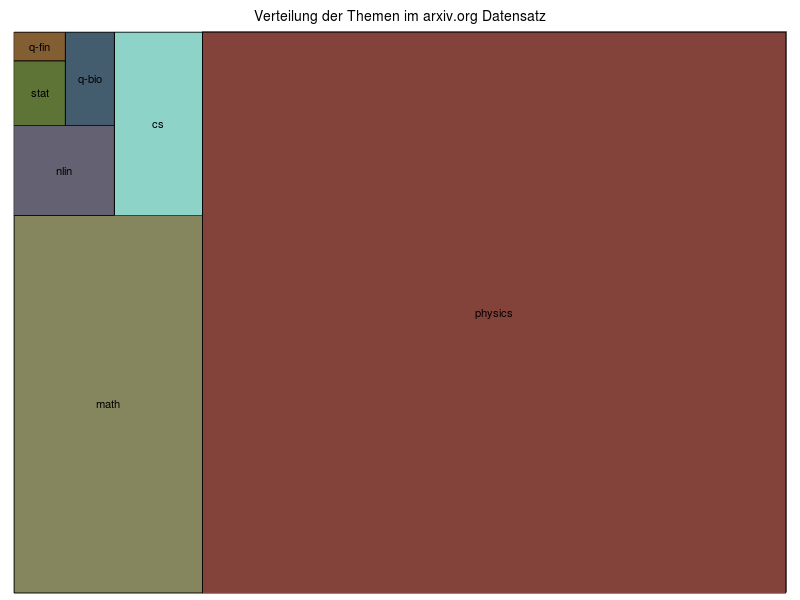
\includegraphics[scale=0.35]{../../visual/treeParent2.png}
	\end{center}
\end{frame}
\begin{frame}[fragile]
	\frametitle{Aufbau des Datensatzes}
	\begin{block}{Header}
		%\begin{Verbatim}[commandchars=\\\{\}, fontsize=\tiny, frame=single]
\PY{n+nt}{<identifier}\PY{n+nt}{>}oai:arXiv.org:0704.0001\PY{n+nt}{</identifier>}
\PY{n+nt}{<datestamp}\PY{n+nt}{>}2007-07-24\PY{n+nt}{</datestamp>}
\PY{n+nt}{<setSpec}\PY{n+nt}{>}\textcolor{red}{\bf{physics:physics}}\PY{n+nt}{</setSpec>}
\PY{n+nt}{<setSpec}\PY{n+nt}{>}\textcolor{red}{\bf{math}}\PY{n+nt}{</setSpec>}
\end{Verbatim}

	\end{block}
	\begin{block}{Metadaten}
		%\begin{Verbatim}[commandchars=\\\{\}, fontsize=\tiny, frame=single]
\PY{n+nt}{<dc:title}\PY{n+nt}{>}Titel des Papers\PY{n+nt}{</dc:title>}
\PY{n+nt}{<dc:creator}\PY{n+nt}{>}Author 1\PY{n+nt}{</dc:creator>}
\PY{n+nt}{<dc:creator}\PY{n+nt}{>}Author 2\PY{n+nt}{</dc:creator>}
\PY{n+nt}{<dc:subject}\PY{n+nt}{>}\textcolor{red}{\bf{Physics - Optics}}\PY{n+nt}{</dc:subject>}
\PY{n+nt}{<dc:subject}\PY{n+nt}{>}\textcolor{red}{\bf{Mathematics - Combinatorics}}\PY{n+nt}{</dc:subject>}
\PY{n+nt}{<dc:description}\PY{n+nt}{>}Description\PY{n+nt}{</dc:description>}
\PY{n+nt}{<dc:description}\PY{n+nt}{>}Comment\PY{n+nt}{</dc:description>}
\PY{n+nt}{<dc:date}\PY{n+nt}{>}\textcolor{red}{\bf{2007-04-02}}\PY{n+nt}{</dc:date>}
\PY{n+nt}{<dc:date}\PY{n+nt}{>}\textcolor{red}{\bf{2007-07-24}}\PY{n+nt}{</dc:date>}
\PY{n+nt}{<dc:type}\PY{n+nt}{>}text\PY{n+nt}{</dc:type>}
\PY{n+nt}{<dc:identifier}\PY{n+nt}{>}http://arxiv.org/abs/0704.0001\PY{n+nt}{</dc:identifier>}
\PY{n+nt}{<dc:identifier}\PY{n+nt}{>}Phys.Rev.D76:013009,2007\PY{n+nt}{</dc:identifier>}
\end{Verbatim}

	\end{block}
\end{frame}

\begin{frame}[fragile]
    \frametitle{Verteilung der Themen in Computer Science}
    \begin{block}{Subjects in CS: Summary}
    	\begin{alltt}\tiny
most frequent items:
                  Computer Science - Information Theory
                                                   6646
             Computer Science - Artificial Intelligence
                                                   3045
      Computer Science - Data Structures and Algorithms
                                                   2878
Computer Science - Networking and Internet Architecture
                                                   2660
           Computer Science - Logic in Computer Science
                                                   2498
                                                (Other)
                                                  58364

element (itemset/transaction) length distribution:
sizes
    1     2     3     4     5     6     7     8     9    10    11    12    13
13906  9209  5443  2802  1351   684   317   173    73    41    16    15     7
   14    15    16    17    19    21    22
    6     5     1     1     1     1     1

   Min. 1st Qu.  Median    Mean 3rd Qu.    Max.
  1.000   1.000   2.000   2.234   3.000  22.000

\end{alltt}

	\end{block}
\end{frame}

\begin{frame}
	\frametitle{Verteilung der Themen in Computer Science}
	\begin{center}
		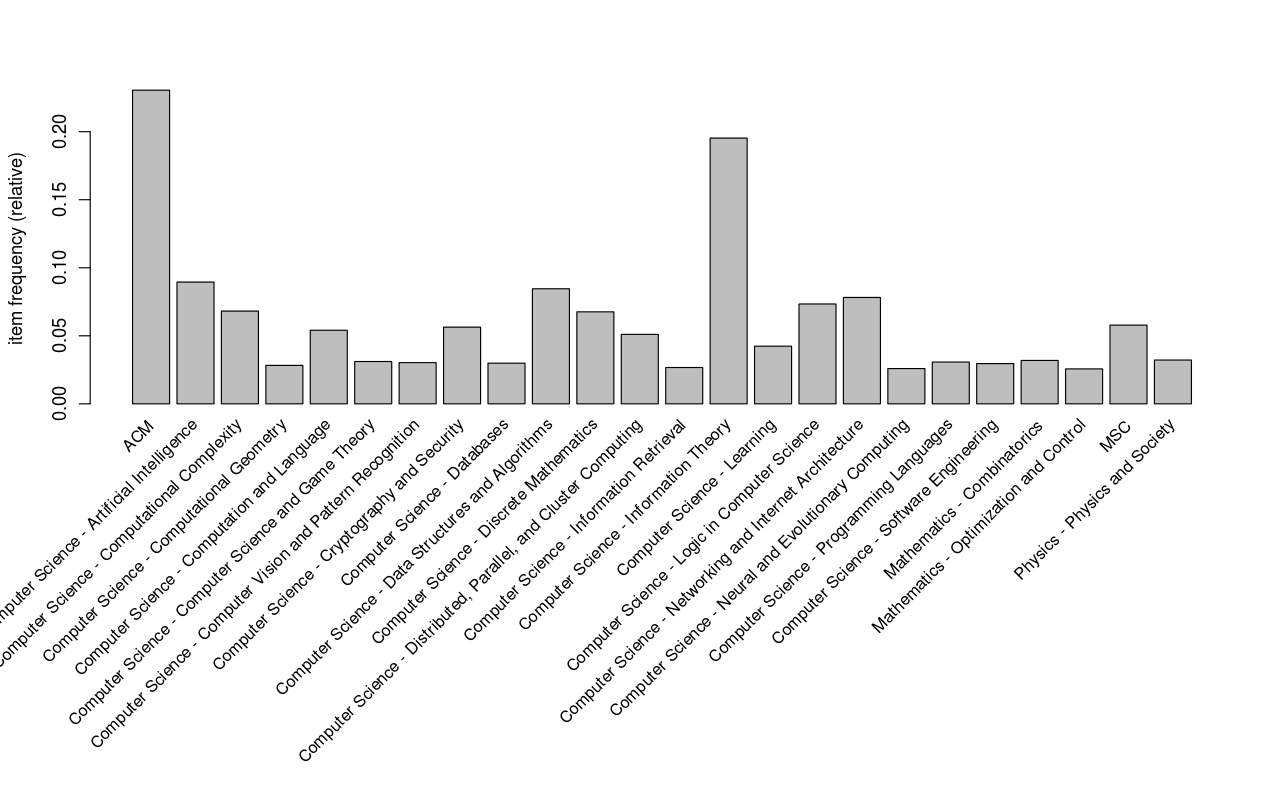
\includegraphics[scale=0.4]{../../visual/csFrequent_filter_acm_and_msc.png}
	\end{center}
\end{frame}
\begin{frame}
	\frametitle{Verteilung der Themen in Computer Science}
    VOSviewer demo
	\begin{center}
		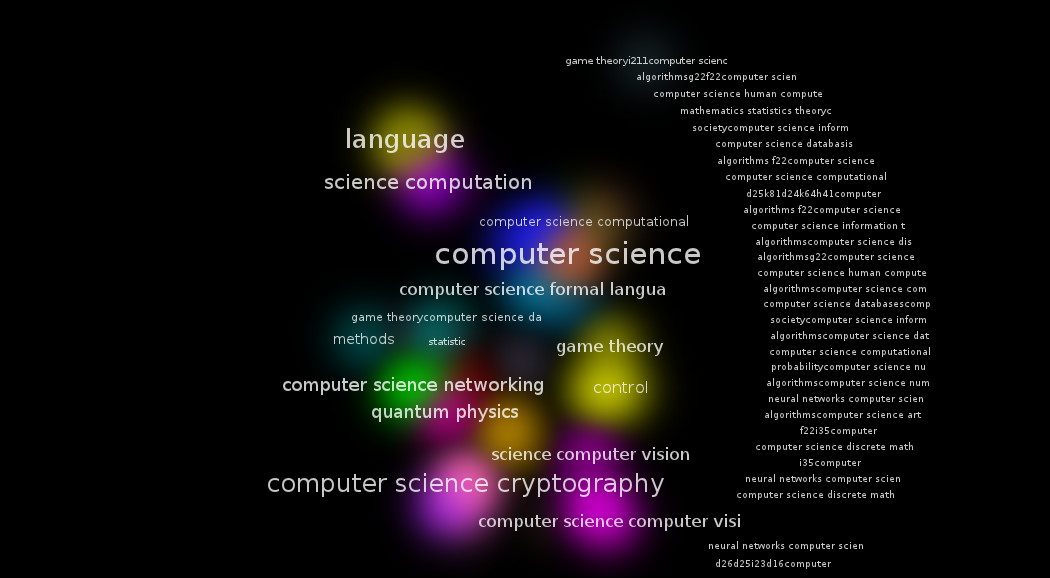
\includegraphics[scale=0.25]{../../visual/cs_subs_cluster_density.png}
	\end{center}
\end{frame}
\begin{frame}
	\frametitle{Entwicklung über die Zeit 1}
	\begin{center}
		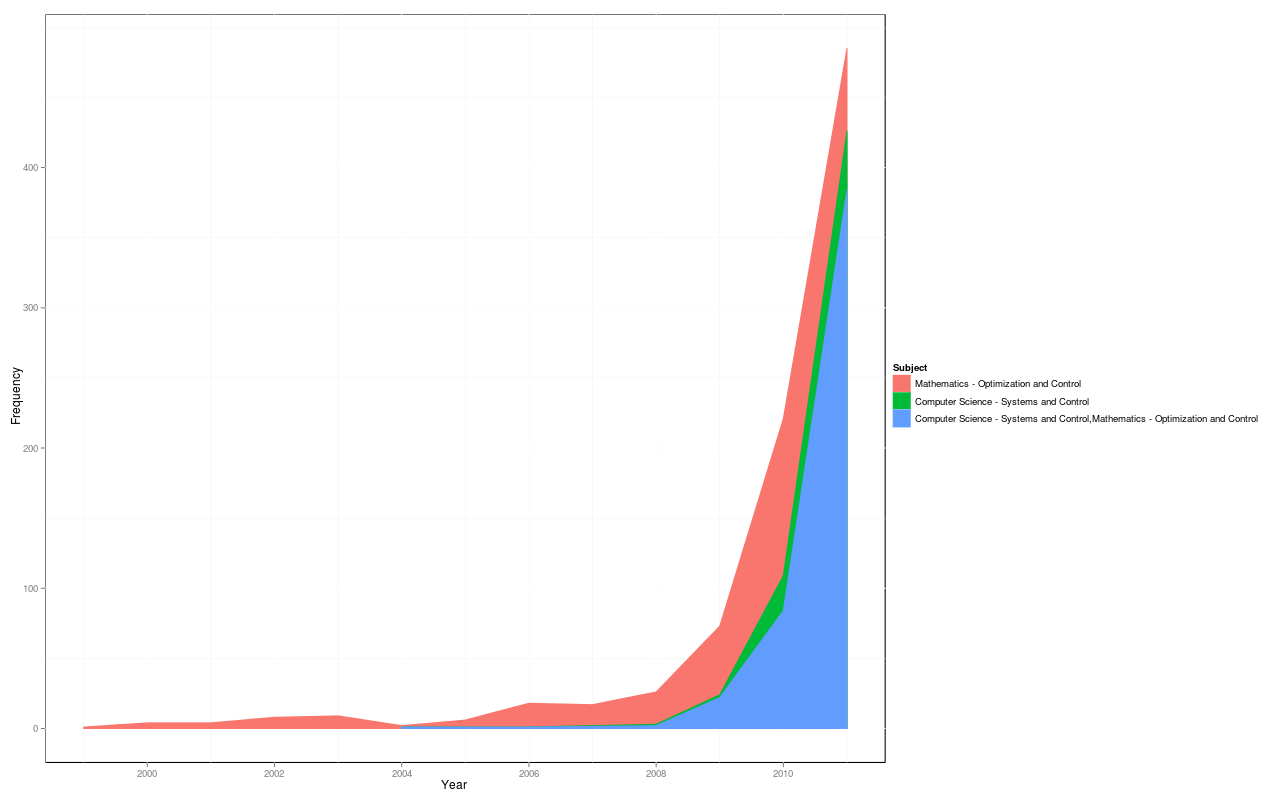
\includegraphics[scale=0.4]{../../visual/trend/csmath.png}
	\end{center}
\end{frame}
\begin{frame}
	\frametitle{Entwicklung über die Zeit 2}
	\begin{center}
		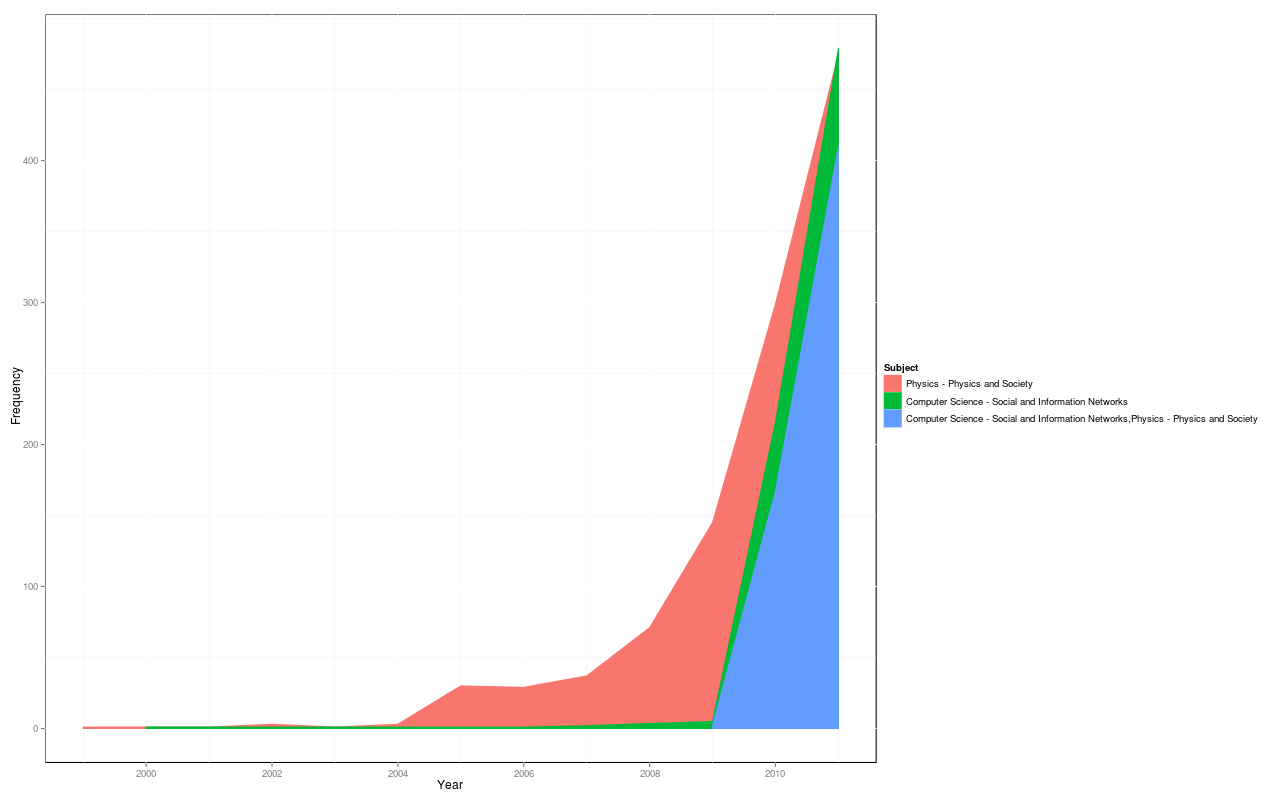
\includegraphics[scale=0.4]{../../visual/trend/csph.png}
	\end{center}
\end{frame}
\begin{frame}
	\frametitle{Entwicklung über die Zeit 3}
	\begin{center}
		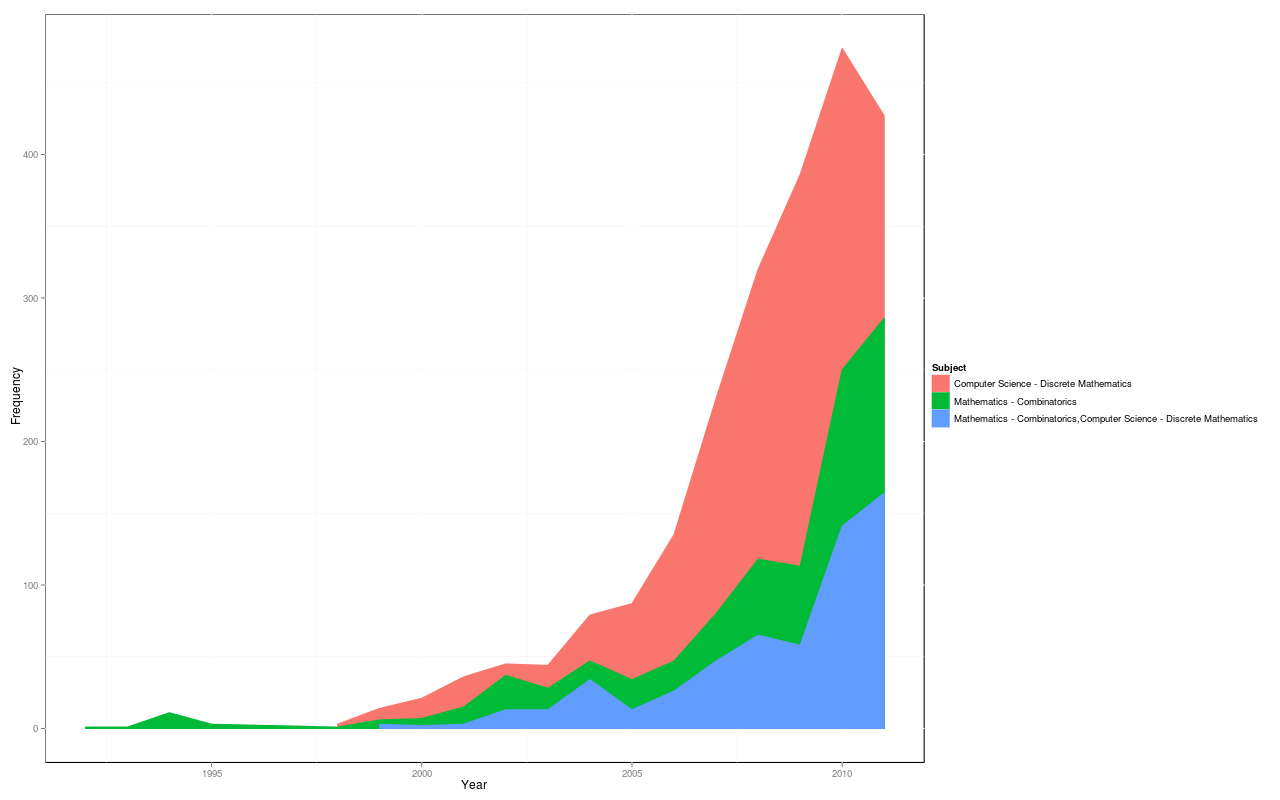
\includegraphics[scale=0.4]{../../visual/trend/combcs.png}
	\end{center}
\end{frame}
\begin{frame}
	\frametitle{Interpretation der Ergebnisse}
    %\begin{block}{Assoziationsregeln - Kenngrößen}
    \begin{center}
        \begin{description}
			\item [Support  ] \hfill \\
                relative Häufigkeit der Menge in den Daten\\
                $supp = \frac{\# gemeinsames Vorkommen Bestimmten Subjects}{\# alle Paper Im Datensatz}$\\
			\item [Konfidenz ] \hfill \\
                Häufigkeit des gemeinsamen Auftretens von X und Y, unter der Bedingung, dass X auftritt\\
                $conf(X\Rightarrow Y) = \frac{supp(X\cup Y)}{supp(X)} $\\

			\item [Lift ] \hfill \\
                Bedeutung der Regel\\
                $lift(X\Rightarrow Y) = \frac{supp(X\cup Y)}{supp(Y)\times supp(X)} $\\
	    \end{description}
    \end{center}
    %\end{block}
\end{frame}
\begin{frame}[fragile]
    \frametitle{Interpretation der Ergebnisse}
    \begin{block}{Arules für supp=0.01}
    	\rowcolors[]{1}{blue!20}{blue!10}
	\begin{tabular}{rccc}
		\tiny \textbf{Regel} &\tiny \textbf{sup} &\tiny \textbf{conf} &\tiny \textbf{lift}\\
		\hline
		\tiny I.2.7 $\implies$ CS - Computation and Language &\tiny 1.2\% &\tiny 90 \% &\tiny 16.9 \\
		\tiny CS- Systems and Control $\implies$ Math - Optimization and Control &\tiny 1.5\% &\tiny 88 \% &\tiny 34 \\
		\tiny Math - Optimization and Control $\implies$ CS - Systems and Control  &\tiny 1.5\% &\tiny 56 \% &\tiny 34 \\
		\tiny CS - Social and Information Networks $\implies$ Physics - Physics and Society &\tiny 1.7\% &\tiny 82 \% &\tiny 25.5 \\
		\tiny Physics - Physics and Society $\implies$ CS - Social and Information Networks &\tiny 1.7\% &\tiny 52 \% &\tiny 25.5 \\
		\tiny F.4.1 $\implies$ CS - Logic in Computer Science &\tiny 1.6\% &\tiny 78 \% &\tiny 10.6 \\
		\tiny Math - Combinatorics $\implies$ CS - Discrete Mathematics  &\tiny 1.7\% &\tiny 54 \% &\tiny 7.9 \\
	\end{tabular}

	\end{block}
    {\footnotesize
        F. - Theory of Computation\\
        F.4. - Mathematical Logic and Formal Languages\\
        F.4.1. - Mathematical Logic\\
        I. - Computing Methodologies\\
        I.2. - Artificial Intelligence\\
        I.2.7. - Natural Language Processing\\
    }
    %\begin{itemize}
            %\item Show rules - results from R
            %\item Visualize - choose an apropriate diagramm
    %\end{itemize}
\end{frame}
\begin{frame}
	\frametitle{Arules für supp=0.01}
	\begin{center}
		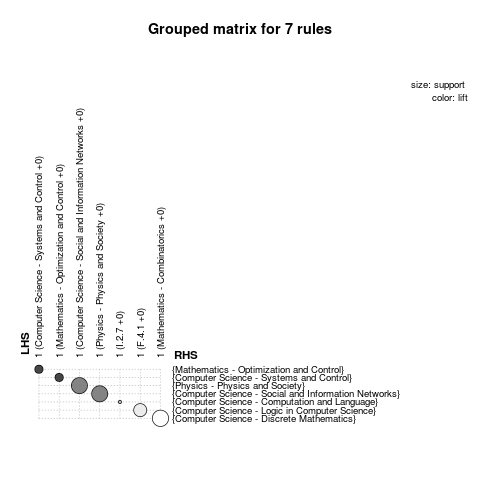
\includegraphics[scale=0.5]{../../visual/plot_matrix_grouped_7rules.png}
	\end{center}
\end{frame}
\begin{frame}
    \frametitle{Interpretation der Ergebnisse}
    \begin{block}{Arules für supp=0.001}
        \begin{itemize}
           \item Same as above
           \item Arules sorted according to supp, conf, lift
        \end{itemize}
    \end{block}
\end{frame}

\begin{frame}
	\frametitle{Mappings zwischen Klassifikationen}
	Top 10(insg. ca. 60)
	\rowcolors[]{1}{blue!20}{blue!10}
	\begin{tabular}{lccc}
		\tiny\textbf{Regel(ACM $\implies$ Arxiv.org)} &\tiny \textbf{Support} &\tiny \textbf{Konfidenz} & \tiny \textbf{Lift}\\
		\hline
		\tiny G.4(Mathematical Software) $\implies$ CS - Mathematical Software & \tiny 0.1\% &\tiny 51\% &\tiny 67.4  \\
		\tiny K.4.m(COMPUTERS AND SOCIETY) $\implies$ CS - Computers and Society &\tiny 0.2 \% &\tiny 96 \%  &\tiny 53.4 \\
		\tiny I.2.9(Robotics) $\implies$ CS - Robotics &\tiny 0.1 \% &\tiny 75 \%  &\tiny 52.1 \\
		\tiny H.3.7(Digital Libraries) $\implies$ CS - Digital Libraries &\tiny 0.3 \% &\tiny 89 \% &\tiny 48.7 \\
		\tiny I.1.2(Symbolic Manipulation - Algorithm) $\implies$ CS - Symbolic Computation  &\tiny 0.1 \% &\tiny 60 \%  &\tiny 41.3 \\
		\tiny I.2.11(Distributed Artificial Intelligence) $\implies$ CS - Multiagent Systems  &\tiny 0.2 \% &\tiny 53 \%  &\tiny 35.9 \\
		\tiny H.5.2(User Interfaces) $\implies$ CS - Human-Computer Interaction &\tiny 0.2 \% &\tiny 58 \%  &\tiny 33.7 \\
		\tiny I.3.5(Computational Geometry) $\implies$ CS - Computational Geometry &\tiny 0.3 \% &\tiny 88 \%  &\tiny 31.2 \\
		\tiny H.2.3(Datebase Managment - Languages) $\implies$ CS - Databases &\tiny 0.2 \% &\tiny 91 \%  &\tiny 30.6 \\
	\end{tabular}
\end{frame}
\begin{frame}
	\frametitle{Einschränkungen für Mappings}
    \begin{itemize}
	\item nur ein Subject auf jeder Seite
	\item Mappings nur von ACM nach Arxiv möglich
	\item Konflikte, durch Mappings von gleichen ACM-Klassen
	\item ab einen Schwellwert für den Lift werden die Mappings zu ungenau 
    \end{itemize}
\end{frame}
\begin{frame}
	\frametitle{Anwendung für Mappings}
    \begin{itemize}
	\item automatische Anpassung von ACM-Klassifikation 
	\item Reduzierung von Subjects pro Paper für Analyse
	\item recommendation 
    \end{itemize}
\end{frame}
\begin{frame}
	\frametitle{Nutzen der verschiedenen Klassifikationen}
    Welche Regeln bleiben übrig, wenn ohne ACM Subjects?\\
\end{frame}
\end{document}
